%%
%% THIS IS A TEST TEX FILE 
%% ========================
%%
\documentclass[12pt,a4paper]{book}

\usepackage{txfonts} % for better Times fonts
\usepackage{epsf}
\usepackage[usenames]{color}
\usepackage{array}
%\usepackage[debugshow]{supertabular}
\usepackage{longtable}
\usepackage{tabularx}
\usepackage{multirow}
\usepackage{graphicx}
\usepackage{cmap}
\usepackage{ugst}
\usepackage[bookmarks=true, bookmarksopen=true, bookmarksopenlevel=0, colorlinks=true, citecolor=red]{hyperref}
%\usepackage[pdftex, linktocpage, bookmarks=true, bookmarksopen=true, bookmarksopenlevel=0, colorlinks=true, citecolor=MidnightBlue, linkcolor=MidnightBlue]{hyperref}
\usepackage{epstopdf}
\usepackage{ifpdf}
\graphicspath{{graphics/}}

\pagestyle{myheadings}

% Special Parameters 
\evensidemargin           0mm
\oddsidemargin            0mm
\parindent                0mm
\parskip                  2mm
\textheight             240mm
\textwidth              160mm
\topmargin              -20mm

%==============================================================================
\begin{document}
%==============================================================================
\sf


\begin{table}[htb]
\centering\small
\caption{Bit stream format for each 20 ms speech frame.}
\begin{tabular}{|c|c|c|} \hline
\bf Parameter     & \bf Parameter & \bf Number \\ 
                  & \bf Number    & \bf of Bits\\
\hline
LAR1              &1    & 6 \\
LAR2              &2    & 6 \\
LAR3              &3    & 5 \\
LAR4              &4    & 5 \\
LAR5              &5    & 4 \\
LAR6              &6    & 4 \\
LAR7              &7    & 3 \\
LAR8              &8    & 3 \\ 
\hline
\multicolumn{3}{|c|}{\bf Sub-frame No. 1} \\ 
\hline
LTP lag           &9    & 7 \\
LTP gain          &10   & 2 \\
RPE grid position &11   & 2 \\
Block amplitude   &12   & 6 \\
RPE-pulse no. 1   &13   & 3 \\ 
$\ldots$          &$\ldots$ &$\ldots$\\
RPE-pulse no. 13  &25   & 3 \\ 
\hline
\multicolumn{3}{|c|}{\bf Sub-frame No. 2} \\ 
\hline
LTP lag           &26   & 7 \\
LTP gain          &27   & 2 \\
RPE grid position &28   & 2 \\
Block amplitude   &29   & 6 \\
RPE-pulse no. 1   &30   & 3 \\ 
$\ldots$          &$\ldots$ &$\ldots$\\
RPE-pulse no. 13  &42   & 3 \\ 
\hline
\multicolumn{3}{|c|}{\bf Sub-frame No. 3} \\ 
\hline
LTP lag           &43   & 7 \\
LTP gain          &44   & 2 \\
RPE grid position &45   & 2 \\
Block amplitude   &46   & 6 \\
RPE-pulse no. 1   &47   & 3 \\ 
$\ldots$          &$\ldots$ &$\ldots$\\
RPE-pulse no. 13  &59   & 3 \\ 
\hline
\multicolumn{3}{|c|}{\bf Sub-frame No. 4} \\ 
\hline
LTP lag           &60   & 7 \\
LTP gain          &61   & 2 \\
RPE grid position &62   & 2 \\
Block amplitude   &63   & 6 \\
RPE-pulse no. 1   &64   & 3 \\ 
$\ldots$          &$\ldots$ &$\ldots$\\
RPE-pulse no. 13  &76   & 3 \\ 
\hline
\end{tabular}
\label{T_order}
\end{table}

% FIGURE TEST

%----------- Begin of FIR filters response: frq for 50 Hz-14 kHz BP filter  ----
\begin{figure}[hbtp]
  \begin{center}
  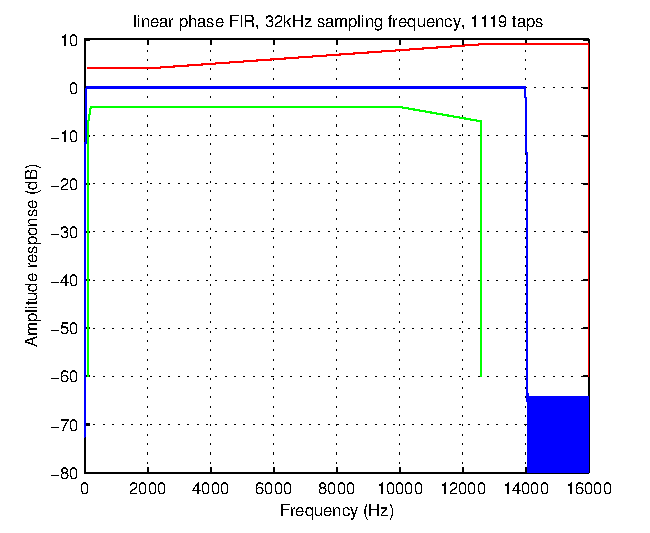
\includegraphics{50-14K}
  \end{center}
  \caption{\SF STL 50 Hz - 14 kHz band limiting filter frequency response for data
               sampled at 32 kHz (factor 1:1).
           \label{50_14k-32k-frq}
          }
\end{figure}
%------------- End of FIR filters response: frq for 50 Hz-14 kHz BP -------------


\end{document}
